\chapter{Introduzione al calcolo parallelo}

Most real world problems need fast, often real time, solutions.

\subsubsection{How to speed up computations}
There are multiple strategies, tipically not mutually exclusive, to speed-up computations.
One of the most effective ones consists of executing multiple operations simultaneously, in \textbf{parallel} or concurrently.

Although there are multiple techniques to achieve parallel computing, the main goal is to overlap the execution of multiple operations or tasks.

\begin{figure}[H]
    \centering
    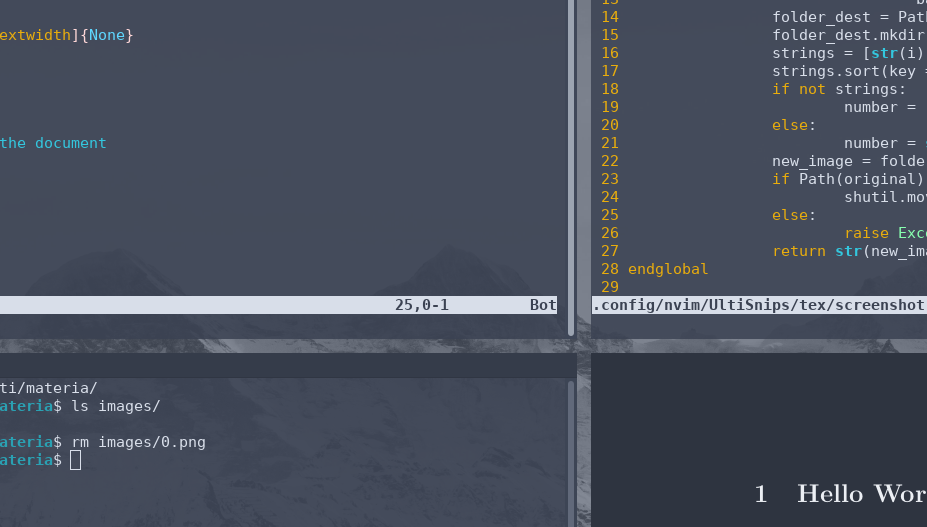
\includegraphics[width=0.8\textwidth]{/home/riccardoob/appunti/sistemi_digitali/images/0.png}
\end{figure}

\section{Dipendenza dei dati e corsa sui dati}

É necessario introdurre concetti base utili durante l'implementazione di operazioni concorrente o parallele.

\subsubsection{Dipendenza dei dati}

La \textbf{dipendenza dei dati}  accade quando un'operazione è dipendente dall'output di un'altra, nel caso di esecuzione sequenziale, questo non è un problema, ma lo diventa in operazioni parallele in quanto una operazione deve rimanere bloccata fino a quando non ha tutti i dati necessari per essere eseguita, magari fornita da operazioni concorrenti.


\subsubsection{Corsa sui dati}

Quando thread multipli accedono alla stessa memoria in modo concorrente, e almeno uno la modifica, si può incorrere in una \textbf{corsa sui dati}. Il risultato non è predicibil, in quanto è influenzato dal timing tra i thread.

\subsection{Soluzioni}

Esistono diverse strategie, che agiscono a livello hardware o software, ma nella maggior parte dei casi, è il design dell'hardware a porre limiti al software.

\subsubsection{Hardware}

\begin{itemize}
    \item aumentare la frequenza
    \item sfruttare pipelining o altre tecniche
    \item permettere operazioni multiple in una singola istruzone
    \item aumentare il numero di core
\end{itemize}

\subsubsection{Software}

\begin{itemize}
    \item eseguire operazioni multiple nella stessa istruzione
    \item distribuire la computazione su CPU multiple
    \item ridurre la dimensione dei dati o effettuare calcoli meno intensi
\end{itemize}

\section{Strategie di design hardware}

\subsection{Aumenare la frequenza}
La soluzione più semplice consiste nell'aumentare la frequenza del clock della CPU.

L'idea è semplice: più alta la frequenza, minore il tempo di esecuzione; tuttavia questo comporta un maggiore consumo di energia, deve quindi essere usata cautamente.

\subsection{Pipelining}
É una soluzione molto efficace che permette di eseguire istruzioni multiple concorrenti, anche se non allo stesso "stadio" di esecuzione (non effettivamente in parallelo).

Si ottiene un CPI (Cycles Per Instruction) minore rispetto alla stessa CPU senza pipelining, tuttavia la sua implementazione richiede più componenti.

In questo caso la dipendenza dei dati diventa un problema, risolvibile però facilmente dalla forwarding unit.

\begin{figure}[H]
    \centering
    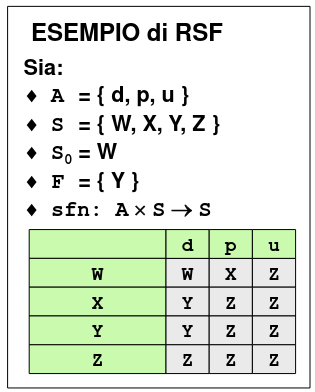
\includegraphics[width=0.6\textwidth]{/home/riccardoob/appunti/sistemi_digitali/images/1.png}
\end{figure}

\subsection{Operazioni multiple in una singola istruzione}
Questa strategia consiste nell'eseguire operazioni (identiche) multiple in una singola istruzione, un singolo registro contiene dati multipli sui quali eseguire l'operazione in parallelo.

\begin{figure}[H]
    \centering
    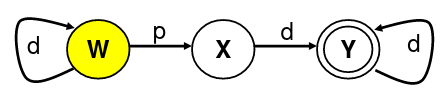
\includegraphics[width=0.8\textwidth]{/home/riccardoob/appunti/sistemi_digitali/images/2.png}
\end{figure}

Single Instruction Multiple Data (SIMD) è una tecnica molto potente e al contempo leggera a livello di implementazione.

\subsection{Aumentare il numero di core}
Consiste nel distribuire il calcolo su più unità di esecuzioni, che siano core o complete CPU.

Questa strategia può essere più efficace e meno costosa rispetto all'aumento della frequenza, tuttavia non è sempre implementabile e sono frequenti i problemi relativi ai dati. 

\section{Strategie di design software}

\subsection{Istruzioni SIMD}
Un buon compilatore è capace di inferire dal codice le possibili computazione parallele per istruzioni SIMD, tuttavia non è facile.

La migliore performance può essere ottenuta organizzando le strutture dati per le SIMD e aggiungere codice assembly nel linguaggio ad alto livello utilizzato, è consigliato applicare questa strategia soltanto alle porzioni più intense del codice.

Questa strategia è efficace quando:
\begin{itemize}
    \item i dati sono organizzati in modo adeguato in memoria
    \item la stessa operazione è applicabile a dati multipli
\end{itemize}

Adatta principalmente all'elaborazione di immagini, contenuti multimediali e segnali, anche se può essere utile anche in altri contesti, come gli algoritmi di sorting.

Se i dati sono appropriamente organizzati in memoria, una singola istruzione può caricare più operandi in un singolo registro multimediale.

\begin{figure}[H]
    \centering
    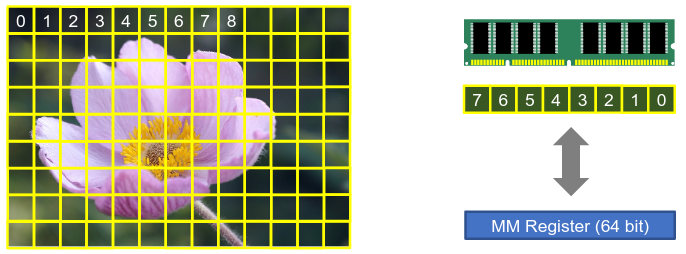
\includegraphics[width=0.8\textwidth]{/home/riccardoob/appunti/sistemi_digitali/images/3.png}
\end{figure}

Una volta caricati dati impacchettati in registri multimediali, una singola operazione può essere applicata a tutti gli operandi.

\begin{figure}[H]
    \centering
    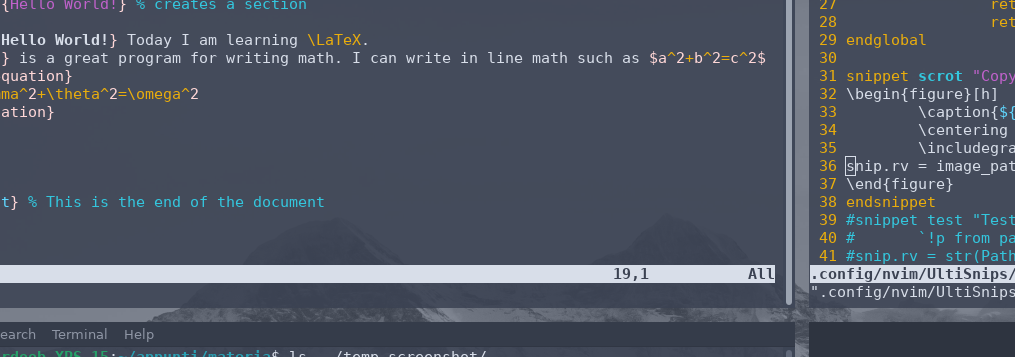
\includegraphics[width=0.8\textwidth]{/home/riccardoob/appunti/sistemi_digitali/images/4.png}
\end{figure}

Ovviamente, un MM register più grande significa un maggiore incremento nella velocità (Intel/AMD up to 512 bit).

\subsection{Sfruttare core multipli}
Invece di agire a livello dell'isruzione/dato è possibile aumentare il parallelismo a livello dei thread, eseguendo sottotask multiple in modo concorrente.

Sfortunatamente, eseguire su core multipli in modo concorrente può risultare in dipendenza dei dati e corsa sui dati portando a risultati non predicibili.

Il motivo risiede nel fatto che ogni thread lavora in modo indipendenta ma su una memoria condivisa che potrebbe contere input, risultati intermedi e risultati di operazioni.

\begin{figure}[H]
    \centering
    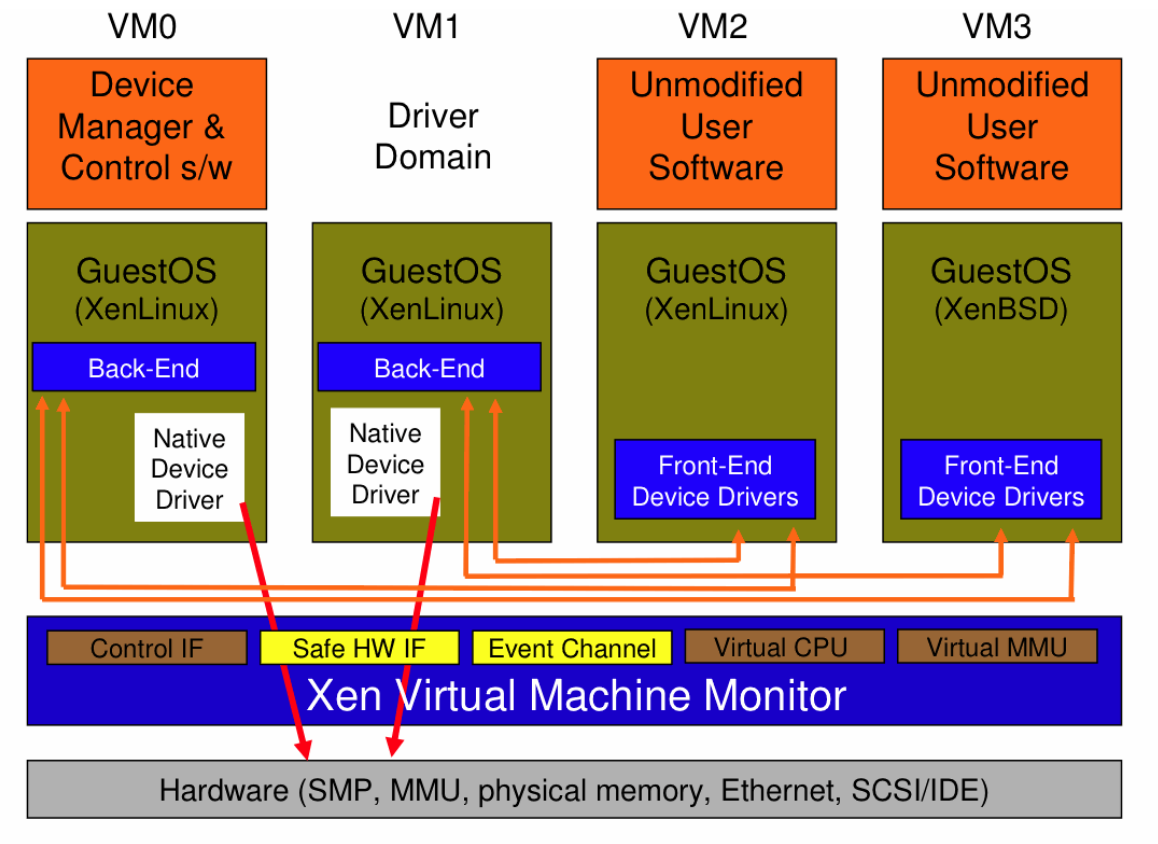
\includegraphics[width=0.7\textwidth]{/home/riccardoob/appunti/sistemi_digitali/images/5.png}
\end{figure}


















